\documentclass{article}
\usepackage[en]{ukon-infie}
\usepackage[utf8]{inputenc}
\usepackage{algorithm2e}
\usepackage{amsmath}
\usepackage{graphicx}
% kann de oder en sein
% kann bubble break, topexercise sein

\Names{Jonas Probst, Simon Giebenhain, Gabriel Scheibler, Clemens Gutknecht}
\Lecture[DLCV]{Deep Learning for Computer Vision}
\Term{WS 2017/18}

\begin{document}
    \begin{ukon-infie}[12.11.17]{1}

		
		\begin{exercise}[p=20]{}
		We decided to combine all training images in one design matrix of shape (number of pixels, 3). Then we compute vector r\_vec which contains the r value for each pixel.  Using both of these and the model parameter vector W containing the $n$ a-values we get our prediction function by simple matrics multiplication on which we compute the loss function which is optimized using the Adam Optimizer. See "solution.py" 	
		\end{exercise}
		
		\begin{exercise}[p=10]{}
        Results only got significantly better up to n=4, after that the loss got a bit higher again but stayed more or less the same.\\
        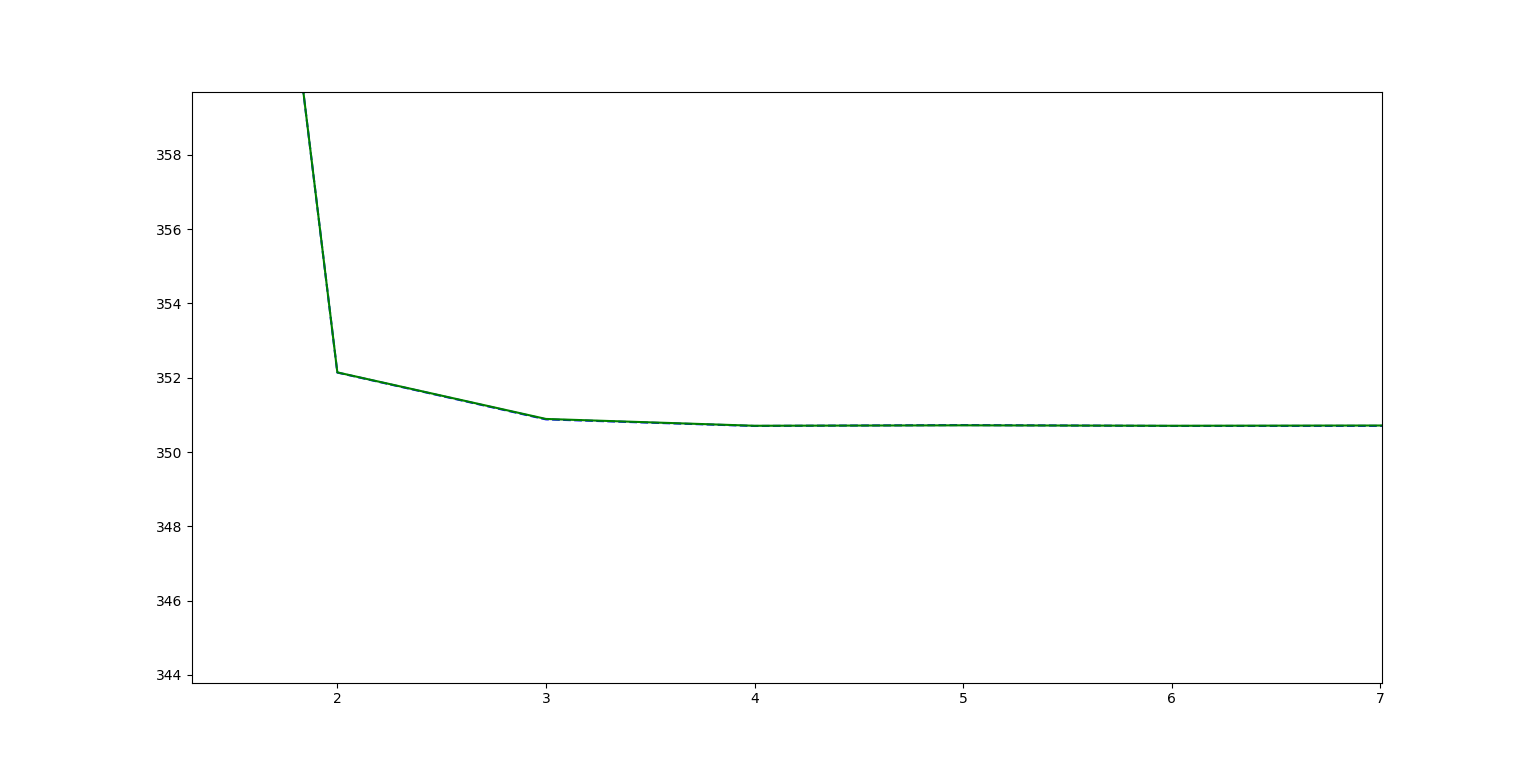
\includegraphics[scale=0.2]{Figure_1}	
        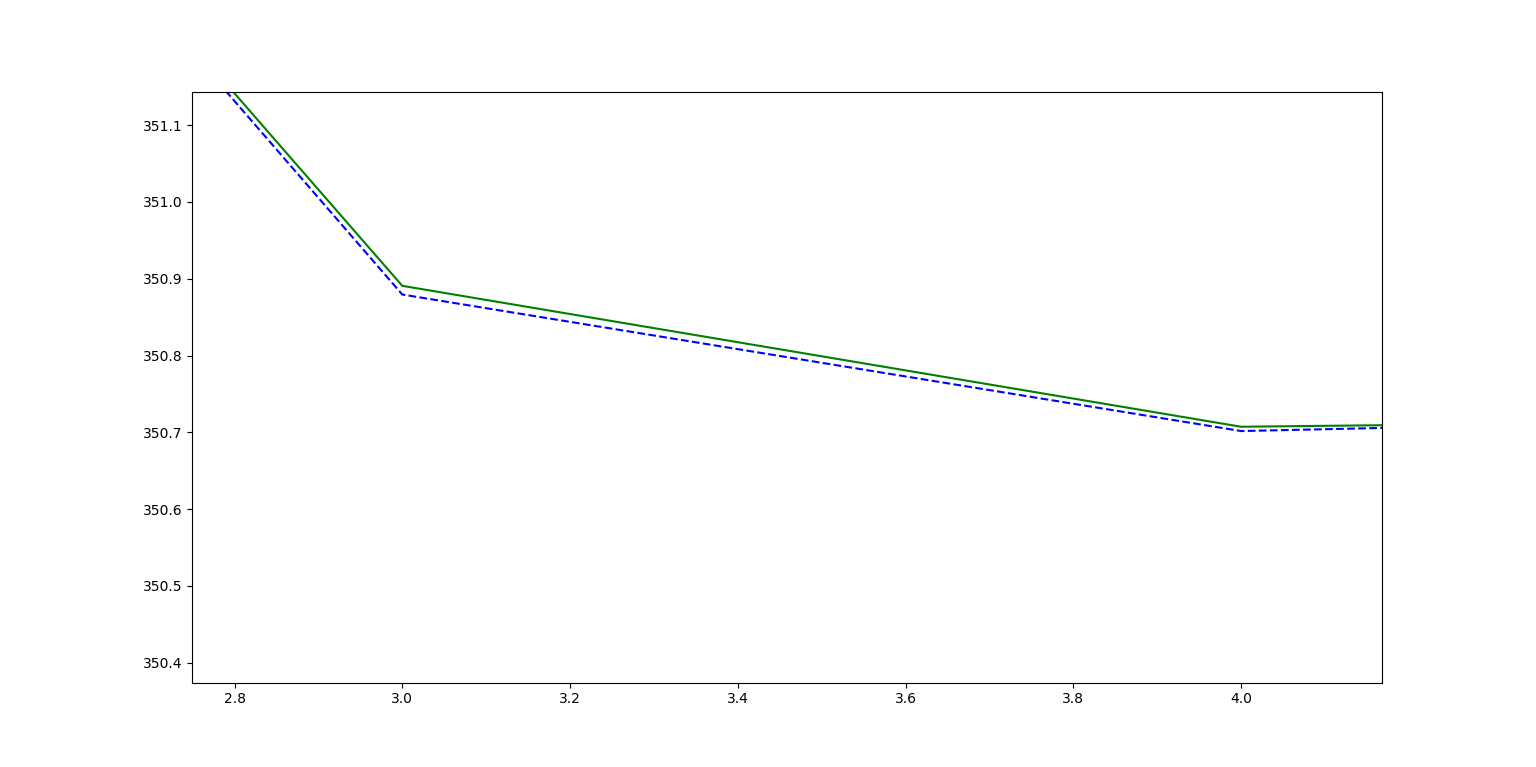
\includegraphics[scale=0.2]{Figure_1-2}
		\end{exercise}
		
		\begin{exercise}[p=10]{}
        	
		\end{exercise}
		
		\begin{exercise}[p=10]{}
        	
		\end{exercise}
		
		\begin{exercise}[p=10]{}
        	
		\end{exercise}
		
		\begin{exercise}[p=10]{}
        	Let $E: \mathbb{R}^3 \rightarrow \mathbb{R}, E(\Theta) = 2\Theta_1^2 + 4\Theta_2 + \text{max}(0, \Theta_2 + \Theta_3)$ be a loss function. In order to perfrom the gradient descent, we first give the gradient of $E$ (which only makes sense if $\Theta_2 + \Theta_3 \not = 0$ ): 
\begin{equation}
\nabla E(\Theta) =
\begin{cases}
\left(
\begin{array}{c}
4 \Theta_1\\
5\\
1\\
\end{array}
\right) & \text{für } \Theta_2 + \Theta_3 > 0 \\
 \left(
\begin{array}{c}
4\Theta_1\\
1\\
0\\
\end{array}
\right) & \text{für } \Theta_2 + \Theta_3 < 0\\
\end{cases}
\end{equation}

With this we compute the following:\\

$\nabla E(\Theta^{[0]}) = 
\left( \begin{array}{c}
8\\
5\\
1\\
\end{array}\right) \Rightarrow \Theta^{[1]} = 
\left( \begin{array}{c}
2\\
1\\
0\\
\end{array} \right)
- \frac{1}{2}
\left( \begin{array}{c}
8\\
5\\
1\\
\end{array} \right) = 
\left( \begin{array}{c}
-2\\
-1.5\\
-0.5\\
\end{array} \right)
$ and\\ 
$\nabla E(\Theta^{[1]}) = 
\left( \begin{array}{c}
-8\\
4\\
0\\
\end{array}\right) \Rightarrow \Theta^{[2]} = 
\left( \begin{array}{c}
-2\\
-1.5\\
-0.5\\
\end{array} \right)
- \frac{1}{2}
\left( \begin{array}{c}
-8\\
4\\
0\\
\end{array} \right) = 
\left( \begin{array}{c}
2\\
-3.5\\
-0.5\\
\end{array} \right)$


		\end{exercise}
		
		\begin{exercise}[p=10]{}
		Let $f: \mathbb{R}^n \rightarrow \mathbb{R}$ and $g: \mathbb{R} \rightarrow \mathbb{R}$ be two differentiable functions. Consider the concatenation $h = g \circ f$. Let $p \in \mathbb{R}^n$ and let $r_f , r_g$ denote the remainders of the linear approximation of $f$ and $g$. Since both $f$ and $g$ are differentiable it holds, that $\lim_{\tau \to 0}\frac{r_f(\tau)}{\tau} = 0$ and $\lim_{\tau \to 0}\frac{r_g(\tau)}{\tau} = 0$ \\
		\begin{eqnarray}
		g(f(p + \tau h)) - g(f(p)) & = & g'(f(p))(f(p + \tau h) - f(p)) + r_g(f(p + \tau h) - f(p)) \\
												& = & g'(f(p))(\tau \nabla f(p)^T h + r_f(\tau)) + r_g(f(p + \tau h) - f(p)) \\
											  & = & g'(f(p))\tau \nabla f(p)^T h + g'(f(p)) r_f(\tau)) + r_g(f(p + \tau h) - f(p))
		\end{eqnarray}
		Now we have still have to show that $lim_{\tau \to 0}g'(f(p)) r_f(\tau)) + r_g(f(p + \tau h) - f(p)) = 0$, this holds because:\\
		$$\lim_{\tau \to 0}\frac{r_f(\tau)}{\tau} = 0$$ and $$\lim_{f(p + \tau h) - f(p) \to 0}\frac{r_g(f(p + \tau h) - f(p))}{f(p + \tau h) - f(p)} = \lim_{\tau \to 0}\frac{r_g(\tau)}{\tau} = 0$$With this we can rewrite (3) to: \\
		
		$$h (p + \tau h) - h(p) = g(f(p + \tau h)) - g(f(p)) = g'(f(p))\tau \nabla f(p)^T h + r_h(\tau)$$ with $\lim_{\tau \to 0}\frac{r_h(\tau)}{\tau} = 0$. \\This matches exactly to the definiton(as a linear approximation) of the gradient/derivative.
        	
		\end{exercise}
		
		
\end{ukon-infie}
\end{document}
